%=========================================================================
% Start of
%=========================================================================
\preClass{Introduction to Exponential Functions}

\begin{problem}
\item Carbon-15 has a half life of about 2.5 seconds. If an object has
  2 grams of carbon-15 in it now, then in 2.5 seconds it will only
  have 1 gram due to its decay. After an additional 2.5 seconds there
  will only be about $\frac{1}{2}$ gram. 

  Suppose that an object has $8.0\times 10^-{6}$ grams of carbon-15,
  and it is placed in a sealed container. Determine how much carbon-15
  is contained in the object at the following times:

  \begin{subproblem}
  \item After 2.5 seconds.
    \vfill
  \item After an additional 2.5 seconds for a total of 5.0 seconds.
    \vfill
  \item After an additional 2.5 seconds for a total of 7.5 seconds.
    \vfill
  \item After an additional 2.5 seconds for a total of 10.0 seconds.
    \vfill
  \end{subproblem}
\end{problem}


\actTitle{Introduction to Exponential Functions}
\begin{problem}
\item A species of bacteria is able to divide every three hours.
  Every three hours each individual bacteria splits into two new
  individuals. Suppose that a colony starts with 10,000
  individuals. For each time below determine the number of bacteria
  and also determine an expression for the total time in terms of the
  three hour time span. (For example, 6 hours = $2\times 3$ hours.)
  \begin{subproblem}
  \item At $t=3$ hours. (Do not simplify the expression.)
    \vfill
  \item At $t=6$ hours. \sideNote{Keep the fractions and do not
      simplify. Look for a pattern.}
    \vfill
  \item At $t=9$ hours.
    \vfill
  \item At $t=n\times 3$ hours where $n$ is an integer greater than or
    equal to zero.  
    \vfill
  \item How many bacteria were in the colony 3 hours before the start
    of the experiment?
    \vfill
  \end{subproblem}

  \clearpage

\item A species of bacteria is able to divide every five hours. That
  is every three hours each bacteria splits into two new
  individuals. After each division, only 75\% of the remaining
  bacteria survive. A colony starts with 10,000 individuals. For each
  time below determine the number of bacteria and also determine an
  expression for the total time in terms of the three hour time
  span. (For example, 6 hours = $2\times 3$ hours.)
  \begin{subproblem}
  \item At $t=5$ hours. \sideNote{Keep the fractions and do not
      simplify. Look for a pattern.}
    \vfill
  \item At $t=10$ hours.
    \vfill
  \item At $t=15$ hours.
    \vfill
  \item At $t=n\times 5$ hours where $n$ is an integer greater than zero.
    \vfill
  \item How many bacteria were in the colony 5 hours before the start
    of the experiment?
    \vfill
  \end{subproblem}

  \clearpage

\item A bank offers a savings account in which the interest is
  compounded 1.5\% annually, and the interest is accrued each
  month. If a person places \$1,000 in an account how much money is in
  the account after $n$ months?
  \textit{Determine the amount of money in the account after the
    first, second, and third months. Do not simplify your results, and
  try to determine the pattern.}

  \vfill

  \clearpage

\item Simplify each expression below.
  \begin{subproblem}
  \item $\frac{3^5\cdot 3^2}{3^4}$
    \vfill
  \item $\frac{2^8}{2^5}$
    \vfill
  \item $\frac{4^2\cdot 2^2}{4^3}$
    \vfill
  \item $5^9\cdot 5^2\cdot 5^{-7}$
    \vfill
  \item $\left(\frac{1}{2}\right)^5 \cdot 2^9 \cdot 2^{-3}$
    \vfill
  \end{subproblem}

\end{problem}

\postClass

\begin{problem}
\item Briefly state two ideas from today's class.
  \begin{itemize}
  \item
  \item
  \end{itemize}
\item A bank offers 1.5\% annual interest compounded weekly (assume 52
  weeks in a year). You will deposit \$5,000 into the account. How
  much money will be in the account at any time?
\item A bank offers 1.5\% annual interest compounded monthly. You will
  deposit some money into an account and wish to have \$25,000 after
  two years. How much money should you deposit?
\item A compound is created that decays over time. It takes four years
  until half of the compound decays in a sample. You wish to store the
  compound for 5 years. How much should you store so that there will be
  4 kg of material at the end of the time period?
\item A colony of bacteria starts with 10,000 individuals. Each
  individual divides into two new individuals every 4 hours. After
  each division only 80\% of the total number of bacteria survive to
  divide later. Determine the number of bacteria present at any time.
\end{problem}


\propertiesTitle{Properties of Exponential Functions}

Exponential functions are used whenever some quantity has a
proportional increase over fixed time spans. An example is a
bacteria population that increases by 100\% every six hours. That
means that every six hours the population doubles. In the diagram
below, a single bacteria starts in a sample. After the first time
period, six hours, there are two bacteria. After another six hours,
a total of 12 hours, there are four bacteria.
In each six hour time period that follows the population doubles.

\begin{minipage}{\linewidth}
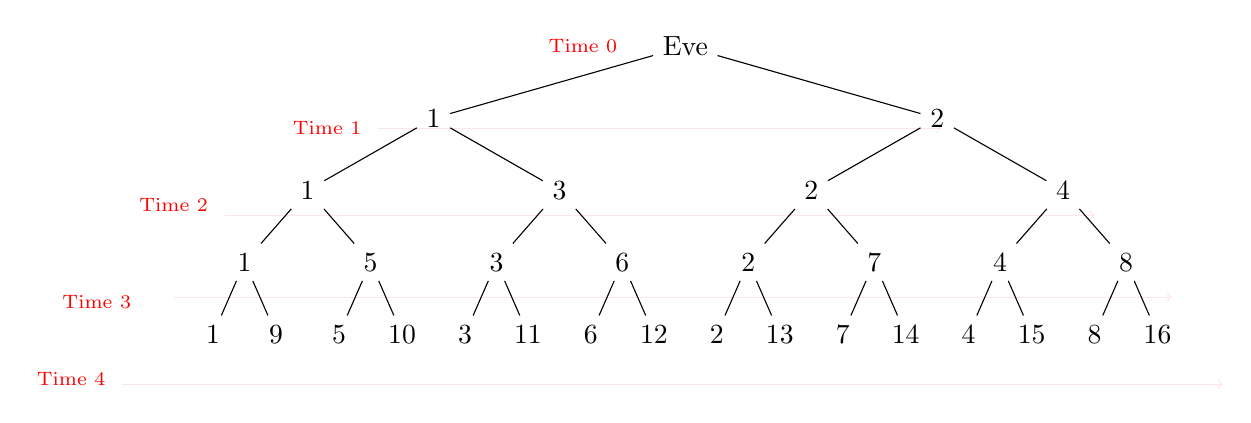
\begin{tikzpicture}[
  scale=0.65,
  grow=down,
  level 1/.style={sibling distance=28em},
  level 2/.style={sibling distance=14em},
  level 3/.style={sibling distance=7em},
  level 4/.style={sibling distance=3.5em},
  level distance = 4em
]
  \draw (-2,0) node [red] {\scriptsize Time 0};
  \draw (-7,-1.6) node [red] {\scriptsize Time 1};
  \draw [->,red!10] (-6,-1.6) -- (5,-1.6);
  \draw (-10,-3.1) node [red] {\scriptsize Time 2};
  \draw [->,red!10] (-9,-3.3) -- (8,-3.3);
  \draw (-11.5,-5.0) node [red] {\scriptsize Time 3};
  \draw [->,red!10] (-10.0,-4.9) -- (9.5,-4.9);
  \draw (-12.0,-6.5) node [red] {\scriptsize Time 4};
  \draw [->,red!10] (-11.0,-6.6) -- (10.5,-6.6);

\node{Eve} %
   child{ node {1}
     child{ node {1}
       child{ node {1}
         child{ node {1}}
         child{ node {9}}
       }
       child{ node {5}
         child{ node {5}}
         child{ node {10}}
       }
     }
     child{ node {3}
       child{ node {3}
         child{ node {3}}
         child{ node {11}}
       }
       child{ node {6}
         child{ node {6}}
         child{ node {12}}
       }
     }
   }
   child{ node {2}
     child{ node {2}
       child{ node {2}
         child{ node {2}}
         child{ node {13}}
       }
       child{ node {7}
         child{ node {7}}
         child{ node {14}}
       }
     }
     child{ node {4}
       child{ node {4}
         child{ node {4}}
         child{ node {15}}
       }
       child{ node {8}
         child{ node {8}}
         child{ node {16}}
       }
     }
   };
\end{tikzpicture}
\end{minipage}

%\clearpage
\vfill

Exponential functions satisfy the algebraic properties given below. In
each example it is assumed that $a$, $b$, and $c$ are constants, and
$a>0$.
\begin{eqnarray}
  a^b \cdot a^c & = & a^{b+c}   \\ [10pt]
  \frac{a^b}{a^c} & = & a^{b-c} \\  [10pt]
  \left( a^b \right)^c & = & a^{b\cdot c}
\end{eqnarray}

Also, $e$ is a constant number, and we define the number $e$ to be
\begin{eqnarray*}
  e & \approx & 2.718.
\end{eqnarray*}

It is common to use the number $e$ as the base for exponentials. The
number $e$ plays the same role as the constant $a$ in the equations
above:
\begin{eqnarray}
  e^b \cdot e^c & = & e^{b+c}   \\ [10pt]
  \frac{e^b}{e^c} & = & e^{b-c} \\  [10pt]
  \left( e^b \right)^c & = & e^{b\cdot c}
\end{eqnarray}



%%% Local Variables:
%%% mode: latex
%%% TeX-master: "../labManual"
%%% End:
